%!TEX root = ../dissertation.tex
\chapter{Introduction}
\label{introduction}
\section{Cholinergic Systems}
\newthought{Nary a process in the mammalian body can commence without participation of cholinergic systems.} Acetylcholine (ACh) was chemically and pharmacologically described by Henry Dale more than 100 years ago\cite{Dale1914}. A short time later, Otto Loewi published the first proof of signal transmission by small molecules: he transferred physiological solutions from electrically stimulated frog hearts to naive hearts and observed their reactions; the solution that provoked a parasympathetic response he proposed to contain a »vagus substance«\cite{Loewi1921}. Finally, in 1929, Henry Dale completed the picture by isolating acetylcholine from mammalian tissue and identifying it as the molecule responsible for the parasympathetic response\cite{Dale1929}. Dale and Loewi's joint effort in »Discoveries in Chemical Transmission of Nerve Impulses« was rewarded with the Nobel Prize in Physiology or Medicine in 1936.

Although we have learned much about cholinergic systems in these past 100 years, our understanding of the mammalian nervous system still is fairly limited. Even when disregarding peripheral nervous systems, the complexity of cholinergic transmission is immense, and a myriad of functions have been attributed to cholinergic circuits in the central nervous system (CNS). Central nervous projections of cholinergic fibres were extensively mapped by M. Marsel Mesulam and others in the 1980s\cite{Mesulam1984}, with a majority of long projection neurons originating in one of the eight cholinergic nuclei, Ch1-Ch8. While many of these anatomical structures have been filled with meaning by associations with both rudimentary as well as higher brain functions, there are still as many cholinergic pathways whose function is entirely unclear (Figure \ref{fig:cholinergicProjections}, from \cite{Lobentanzer2019}).

This holds particularly true for the only recently discovered cortical cholinergic interneurons, which, in comparison to their projecting counterparts, are very small and numerically vastly inferior to other neuron types in the cortex. Thus, their detection and analysis with current methods is challenging. 

\begin{figure}
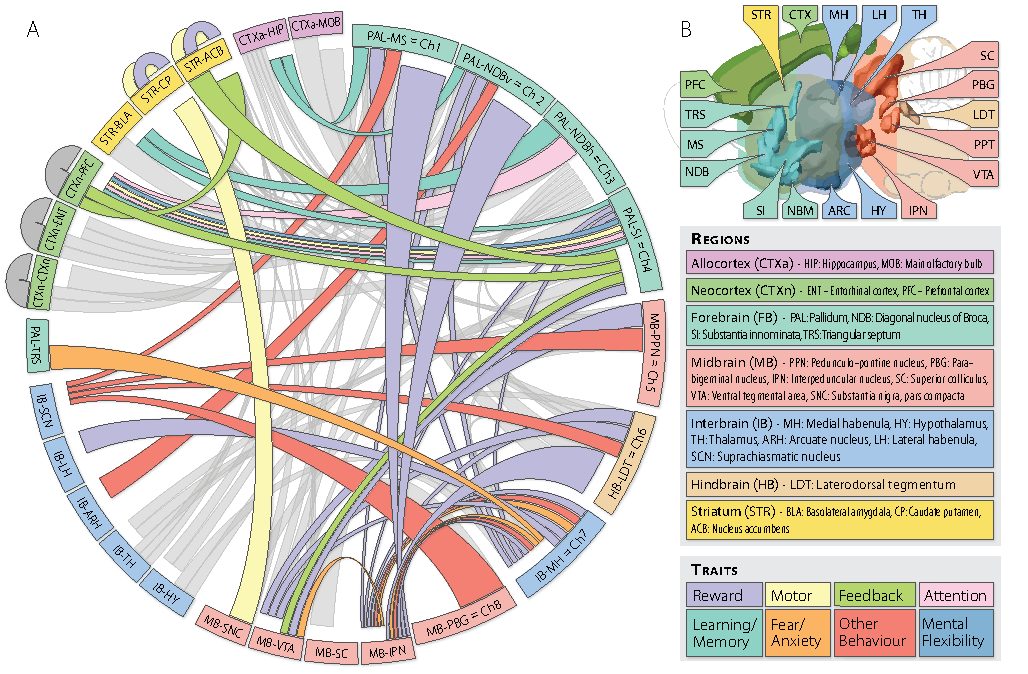
\includegraphics[width=\textwidth]{figures/projections}
\caption[Short figure name.]{This is a figure that floats inline and here is its caption.
\label{fig:cholinergicProjections}}
\end{figure}

Disease? Subsection for disease?

\subsection{Neurokines}
In comparison to the widely studied cholinergic projection neurons originating in the basal forebrain (Ch1-Ch4) that are known to depend on a retrograde survival signal by means of neurotrophic growth factor (NGF), trophic influences on other cholinergic populations such as the cortical interneurons are unclear.  NGF was described by Rita Levi-Montalcini in the 1950s as the first known instance of trophic peptides required for the survival of sympathetic ganglia\cite{Levi-Montalcini1960}, and the dependence of basal forebrain cholinergic neurons on retrograde NGF signalling was discovered in the 1980s\cite{Hefti1986}.

A second group of trophic peptides with cholinergic implications are the so-called »neurokines«; the name results from the fact that this particular subgroup of cytokines has been associated with neuronal function in the central and peripheral nervous systems. Most prominently they include the ciliary neurotrophic factor (CNTF), leukaemia inhibitory factor (LIF), and interleukin 6 (IL-6), all of which coincidentally have been known under the acronym CDF. In the end of the 1980s, two groups of scientists (McManaman\cite{McManaman1988} and Rao\cite{Rao1992}) independently identified proteins in extracts of muscle fibre that induced a differentiation of neurons towards a cholinergic type, and thus termed these proteins »choline acetyltransferase development factor« or »cholinergic differentiation factor« (both abbreviated CDF). Only later, through sequencing of the peptides, it became known that they had in fact discovered two distinct neurokines, LIF (Rao) and CNTF (McManaman, personal communication). IL-6, on the other hand, is abbreviated CDF for an entirely different reason: in this case it is short for »CTL (cytolytic T lymphocyte) differentiation factor«.

CNTF, LIF, and IL-6 convey their impact on neuronal activity through a partly redundant neurokine receptor pathway. There are two basic types of neurokine receptors: soluble and transmembrane. The primary receptors for CNTF (CNTFR) and IL-6 (IL6R) are soluble proteins that are secreted into the extracellular space and, upon binding of a neurokine, bind to transmembrane receptor dimers on the cell surface. These transmembrane receptors are the LIF-receptor (LIFR) and the »IL-6 signal transducer« IL6ST, also known as gp130. Every neurokine has its preferred constellation of soluble and transmembrane receptors: CNTF bind to the soluble CNTF receptor and a dimer consisting of one gp130 and one LIFR protein; IL-6 binds to the soluble IL6R and a dimer from two units of gp130; LIF does not usually bind a soluble receptor but rather binds immediately to a dimer comprising one of each gp130 and LIFR; however, there is significant redundancy and crosstalk between those systems\cite{Rawlings2004,Nathanson2012}.

All receptor constellations result in a main effect of activation of the JAK/STAT cascade. More specifically, neurokines can activate janus kinases (JAK) 1 and 2 or the homologous tyrosine kinase (TYK) 2, and successively »signal transducer and activator of transcription« (STAT) isoforms 1, 3, 5A, and 5B, which then convey a multitude of cellular effects (e.g. in immunity or differentiation) through transcriptional activation. The STAT cascade is inherently self-limiting in that it usually leads to expression of transcription factors that serve as repressors of the STAT genes (XXX).

\todo{FIGURE STAT}

%Neuronal activity is profoundly modified by cytokines

%Li Gan - NFkB activation by tau
% - Ikkbeta knockout corrects STAT1 DE

%Oleg Butovsky - TGFbeta as master glia regulator

\section{Transcriptional Connectomics}
\newthought{No matter their location, cholinergic neurons are defined by their ability to synthesise ACh and release it to neighbouring cells to a certain effect.} To fulfil this capacity, two particular proteins are essential: the choline acetyltransferase (ChAT) to synthesise ACh from choline and acetyl-Coenzyme A, and the vesicular acetylcholine transporter (vAChT, official gene symbol SLC18A3), which concentrates ACh in vesicles for later release. A notable genetic feature connects these two proteins beyond their functional association: the small \textit{SLC18A3} gene (\mbox{2 420} nucleobases) sits inside the first intron of the \textit{CHAT} gene and thus is already included in its primary transcript, and is subject to the \textit{CHAT} promoter. However, oftentimes the (mature) transcript levels of \textit{CHAT} and \textit{SLC18A3} mRNA seem to be independently regulated; from the perspective of the organism, the possibility of differential regulation between these two genes makes sense. Since \textit{SLC18A3} does not possess its own promoter, this differential regulation has to be conveyed epigenetically. 

This dissertation deals in large parts with approaches aiming to decipher these interactions; and while its primary topic revolves around cholinergic systems, the methods described in the following are designed to be applicable to the entirety of the genome/epigenome. Four particular types of cellular actors are subject of these methods and therefore will be briefly introduced: genes in the classical sense as the conveyors of cellular function by encoding for proteins; transcription factors, a subclass of protein coding genes that are able to regulate the expression of other genes; microRNAs (miRNAs), a class of small non-coding RNA that has been known for approximately two decades and is reasonably well described functionally and mechanistically; and transfer RNA fragments (tRFs), a second class of small non-coding RNA that has only recently been rediscovered and is significantly less well described regarding its functionality.

Where to put:\todo{where goes this?}

Distinguish neuronal connectomics from transcriptional connectomics

For the sake of simplicity, all descriptions of genomics and transcriptomics matters, genes, miRNAs, and tRFs in this dissertation are to be seen in the context of Homo sapiens, unless explicitly stated otherwise.

\subsection{Transcription Factors} \label{intro:TFs}
Transcription factors (TFs) were among the first intracellular regulatory mechanisms to be discovered (the earliest article referencing the term »transcription factor« in its title on PubMed was published in 1972). TFs commonly translocate from the cytosol into the nucleus upon activation (often by phosphorylation), where they bind specific DNA sequences that usually range in size from 6 to 12 nucleobases. The regions containing these binding sites (about 100 - 1 000 bases in size) determine the effect upon binding, which can be one of two main modes: either a promoter, leading to an increased activity of transcription in the downstream vicinity of the binding site, or a repressor, having the opposite effect. 

There exists a vast body of knowledge on TF interactions with genes, mostly due to the long period of time since their discovery and the multitude of scientific publications, most often studying single TFs and their interactions with few genes, but cumulatively curated by several organisations. One of the currently largest curations of TF data, TRANSFAC, saw its original release in 1988. While these curation efforts can be extensive, they may present with serious bias towards particular TFs that might hold more scientific interest and thus are published far more frequently than others. Recently, comprehensive efforts have extended the available data significantly. Driven by the advent of RNA sequencing, computational approaches have become able to not only comprehensively predict TF-gene interactions, but to do so in a highly tissue-specific manner (see \ref{database:TF}). The human body is estimated to express up to 2 600 distinct DNA-binding proteins, most of them presumed TFs\cite{Babu2004}, although other studies give lower estimates. 

\subsection{microRNAs} \label{intro:miRNAs}
While the first endogenous »small RNA with antisense complementarity« was described in 1993\cite{Lee1993}, miRNAs were only recognised as a distinct regulatory class of molecules in the early 2000s. They are typically between 18 and 22 nucleobase-long, single stranded RNA fragments, and their function is now largely undisputed: miRNAs serve as targeting molecules for a protein complex whose primary purpose is to repress translation of mRNA, and, in some cases, lead to mRNA degradation. The complex, therefore, is called »RNA-induced silencing complex« (RISC); central to its function is the family of Argonaute (Ago) proteins, which can bind the mature miRNA and orient it for interaction with its targets. Guidance of RISC to the target mRNA is generally mediated via sequence complementarity between miRNA and the targeted mRNA. Specifically, a »seed« region, usually bases 2-8 on the miRNA, is mainly responsible for the interaction; in case of perfect complementarity of this seed to the mRNA sequence, the interaction is considered »canonical«.

In early miRNA research, the 3' untranslated region (UTR) of the mRNA was believed to contain most miRNA binding sites due to its greater accessibility (i.e., the lack of active ribosomes); however, cumulative recent reports suggest that binding inside the coding region of the mRNA is a regular occurrence\cite{}. The rules governing miRNA binding to target sequences show considerable flexibility; a recent study shows about 30\% of analysed relationships to be of »non-canonical« nature\cite{}. In those cases, seed pairing with the mRNA is often imperfect. To ameliorate this loss of stability, compensation occurs typically by a secondary complementary structure after a small gap of non-complementary bases, leading to a »bridge«-type constellation. FIGURE? This flexibility has implications in applications involving targeting algorithms; those that consider only the seed region are more prone to false negatives than models that consider, for instance, the free energy of the whole molecule (see \ref{database:miRNA}).

miRNAs, similar to coding genes, are transcribed from loci on the genome, many inside introns or even exons of coding genes\cite{Rodriguez2004}. The primary transcript (primary miRNA or pri-miRNA) typically contains a hairpin-like structure that usually results in a double-stranded molecule because of internal complementarity, and can contain up to six mature miRNAs. This hairpin structure is recognised by the DGCR8 protein (DiGeorge Syndrome Critical Region 8, in invertebrates called »Pasha«); the complex then associates with the RNA-cleaving protein »Drosha«, which removes bases on the opposite side of the hairpin, creating a miRNA precursor (or pre-miRNA), which is subsequently exported from the nucleus by the shuttle protein Exportin-5. In a final step in the cytosol, the RNAse »Dicer« removes the loop joining the 3' and 5' arms of the pre-miRNA, resulting in a duplex of mature miRNA, about 20 nucleotides long. Initially, it was thought to contain only one active miRNA, resulting in a designation of »miRNA*« for the complementary strand (commonly, the strand with lower expression). However, this notion has been disproven, and to reflect the possibility of both strands performing miRNA functions, nomenclature has changed to specify the arm of the pre-miRNA from which the mature form originates (suffix »-3p« for the 3' arm, and »-5p« for the 5' arm).

miRNAs are organised and curated by means of a periodically updated web-based platform, miRBase\cite{Kozomara2019}. For Homo sapiens, miRBase v21 contains 2 588 mature miRNAs from XXX precursors. Evolutionarily, the miRNA repertoire has grown from rodents to primates, resulting in a number of primate-specific miRNAs that may convey additional function. miRNA nomenclature is organised\cite{Ambros2003} in a way that assigns evolutionarily conserved miRNAs the same designation (number) in all species in which they are expressed. In their full names, a prefix stating the organism of origin is added; for example, hsa-miR-125b-5p (for Homo sapiens) and mmu-miR-125b-5p (for Mus musculus) share the same sequence and most of their functionalities.

Disease?

miRNA genes, in the same way as protein coding genes, can also be subject to promoters and repressors, adding another layer of expression control by TFs. However, these TF-miRNA relationships are far less well described than common coding gene interactions, because miRNAs due to their shortness are not amenable to many standard gene expression assay forms. Estimation of the number of distinct targets of any one miRNA varies widely; however, it is generally accepted to not be less than several dozen targets per miRNA, and up to thousands of genes per miRNA (although that estimate might be overenthusiastic).

Prediction?

\subsection{Transfer RNA Fragments}
Self-plagiarised: Recent studies have shown transfer RNA (tRNA) to be a major source of small noncoding RNA\cite{Cole2009,Lee2009}, including tRNA halves (tiRNAs) and smaller tRNA fragments (tRFs). tiRNAs derive from either end of the tRNA, and are created by angiogenin cleavage at the anticodon loop\cite{Yamasaki2009,Ivanov2011}. Smaller fragments are derived from the 3’ and 5’ ends of the tRNA (3'-tRF/5'-tRF) or internal tRNA parts (i-tRF), respectively, and may incorporate into Ago protein complexes and act like miRNAs to suppress their targets\cite{Burroughs2011,Kumar2014}.

However, there is considerable controversy about the generalisation of tRF functions, as distinct publications discover very different and sometimes opposing mechanisms of action for their respective fragments. An obvious assumption is the miRNA-like functionality, at least for those tRFs that are in the length range of miRNAs. There have been several instances of tRFs proven to act as miRNA-like suppressors of translation in a RISC-associated manner\cite{Kumar2014}, and of Dicer playing a large part in their biogenesis\cite{Cole2009}. There are even instances of small RNA molecules previously mislabeled miRNAs that have been discovered to actually be tRNA-derived, such as miR-1280\cite{Huang2017}.

On the other hand, multiple groups have identified tRFs to function not in an antisense-complementary manner, but by homology aspects. A valine-derived tRF was found to regulate translation by competing with mRNA directly at the binding site at the initiation complex and thereby displacing the original mRNA, leading to its translational repression\cite{Gebetsberger2017}. Others have found multiple classes of tRFs derived from glutamine, aspartate, glycine, and tyrosine tRNAs, that displace multiple oncogenic transcripts from an RNA-binding protein (YBX1), conveying tumor-suppressive activity\cite{Goodarzi2015}. Most counterintuitive is the recent finding of a tRF proven to bind to several ribosomal protein mRNAs and enhancing their translation, and, when specifically inhibited, leading to apoptosis in rapidly dividing cells\cite{Kim2017}.  

History?

There is no consistent nomenclature yet to describe and organise tRFs, which are by nature more heterogeneous than miRNAs; considering their biogenesis, one tRNA molecule can be the origin of several hundred distinct tRF molecules. Multiple approaches are common in current literature, most prominently tRFs are tied to the parent tRNA and the amino acid coded for by this tRNA. For example, the 22-nucleotide-long LeuCAG3′ tRF (meaning: a fragment of 22 bases starting at the 3' end of the leucine-carrying tRNA with anticodon »CAG«) was shown to play an important role in regulating ribosome biogenesis\cite{Kim2017}. Since there is no repository of the likes of miRBase yet, this approach can be cumbersome for replication purposes, and explicit statement of the exact sequence of each fragment is a must in publication. For this reason, the approach of Loher and colleagues\cite{Loher2017} might be preferable: they propose the generation of a "license plate" based on the sequence of the fragment directly, composed of the prefix »tRF«, the length of the fragment, and a custom oligonucleotide string encoding (e.g., »B3« stands for »AAAGT«). This way, tRF names are unique and unmistakably linked to the sequence, nomenclature is species-independent, and tRNA origin can be quickly determined by sequence lookup.

Disease?

? Levels of tRFs may be modulated even more rapidly than levels of miRs, since tRNA molecules are very abundant in the cell and generation of mature tRFs requires only enzymatic degradation of tRNA but no de-novo transcription of the molecule in the nucleus (citation).

\subsection[Nested Multimodal Transcriptional Interactions - The Need for Connectomics]{\nopagebreak{Nested Multimodal Transcriptional Interactions\\ \qquad \qquad - The Need for Connectomics}}
For every scientist trying to explain the cooperation between only these few factors in light of how genotype results in phenotype, or how dysregulation of any one factor leads to loss of homeostasis and eventually disease, multiple levels of obstacles have to be overcome. The ultimate aim of any such approach is the generation of a robust model for the studied phenomenon; the theoretical and practical hurdles to be surmounted to reach this goal are many. Theoretically, the more we know about the functioning of these intertwined systems, the more we understand how much there is still to learn. 

For example, only recently it has become clear how complex transcriptional regulation by means of TFs really is, and, incidentally, the two systems studied foremost in this dissertation (nerve and immune cells) are the two most transcriptionally complex systems in any mammal. Through study of comprehensive genomic information of 394 tissue types in approximately 1 000 human primary cell, tissue, and culture samples (from the FANTOM5 consortium) it was estimated that genes in immune and nervous cells are controlled by a mean of 12 and 10 TFs each, and that TFs in nervous and immune cells influence expression of a mean of 175 and 160 genes, respectively (see \ref{database:TF}). 

Similarly, it has been found that miRNAs, particularly in the nervous system, possess a much higher tissue specificity than coding genes, resulting in an expression landscape that varies widely between individual neuron types that are in close proximity in the brain. With the exception of single cell sequencing, no modern analysis method is capable of a resolution appropriate for accurate characterisation of these expression patterns, resulting in extinction of the signal of miRNAs that are not expressed consistently across cell types (similar to »housekeeping« genes) because of statistical interference. Very recent studies show that miRNA-gene co-expression networks are tightly linked to cell types in the nervous system, and that groups of miRs as functional modules associate with particular phenotypes in developmental and mature states\cite{Nowakowski2018}. This functional association with cell phenotype was found in quality comparable to the expression patterns of TFs, yet in quantity conveys smaller impact and thus is thought to be a fine-tuning mechanism, subtle and precise in purpose. 

Another aspect of the tissue specificity of CNS-associated miRNAs is the high likelihood of underrepresentation for those very specifically expressed miRNAs. Adding to the problem is the experimental bias towards rodent models when it comes to thorough studies of the CNS, where human or other primate samples are a rarity compared to rats or mice. Assessments of the numbers of yet unknown novel primate- and tissue specific miRNAs estimate their magnitude in the thousands\cite{Londin2015}, resulting in an effective doubling of currently known miRNAs.

These high numbers of potentially interacting players present computational challenges: If estimating the number of expressed genes in a human cell at 20 000 (and the number of TFs at a low 1 000), this makes for an estimated minimum of 200 000 »real« interactions in the possible $ C = \frac{1\,000!}{10!(1\,000-10)!} \cdot 20\,000 $, which practically equals infinity; this is without accounting for different tissue types or cell states (e.g., differentiation or disease). Similarly, the amount of mature miRs (2 588 in miRBase v21) and their ability to target even more distinct transcripts than TFs with one single molecule present immense computational requirements for even listing all possible or actual relationships. An interaction table describing targeting of genes by miRNAs in one type of tissue has $ 2\,588 \cdot 20\,000 = 51\,760\,000 $ individual fields.

Combining all aspects of transcriptional interaction presents additional challenges. A simple model system to visualise (in only one type of cell) the interaction of TFs targeting genes, and of miRNAs targeting genes as well as TFs, contains about 20 000 genes (a subset of which of the size of about 2 000 are TFs), 2 588 mature miRNAs, and a total of $ 2\,588 \cdot 20\,000 + 2\,000 \cdot 20\,000 = 91\,760\,000 $ potential interactions. In standard application scenarios, such as the generation of an interaction network around a group of genes (e.g., the cholinergic genes), the processing requirements grow linearly with each added interaction partner, and exponentially with every regulatory layer that is added. 

Practically, this information has to be provided, gathered, and integrated, which further multiplies the amount of storage and processing power required. miRWalk 2.0, a collection of miRNA interaction data, has collected 12 of the most popular miRNA-targeting prediction datasets, each of which has their strengths and weaknesses (see \ref{database:miRNA}). Experimentally validated interactions (e.g. as collected in DIANA TarBase or miRTarBase) are gold standard, but far from comprehensive and strictly speaking only relevant for the cellular context in which the experiment was originally performed; there are also different evidence qualities to be accounted for, depending on the type of experiment performed. Ideally, all of these data are still accessible when performing the analysis, so a database created for this purpose should be able to incorporate all this information without any data loss while still remaining feasible in terms of computation time as well as space and working memory requirements. 

This dissertation will first describe the creation of such a database and what has been learned during its various stages, and then go on to apply the database to different biological problems from real world experiments, such as the cholinergic differentiation of male and female cultured cells, or the blood of stroke victims.